\documentclass[10pt]{article}
\usepackage[a4paper,margin=0.72in,headheight=21pt]{geometry}
\usepackage{mathptmx,graphicx,array,longtable,color,fancyhdr,url}
\definecolor{BorderBlue}{RGB}{38,91,145}\definecolor{PaleBlue}{RGB}{233,241,249}\definecolor{DarkInk}{RGB}{28,36,45}
\color{DarkInk}\setlength{\parindent}{0pt}\setlength{\parskip}{5pt}
\pagestyle{fancy}\fancyhf{}\lhead{DOC-2-033 combined R1/R2 package}\rhead{Packaging-only backfill}\cfoot{\thepage}
\renewcommand{\headrulewidth}{0.8pt}\renewcommand{\headrule}{\hbox to\headwidth{\color{BorderBlue}\leaders\hrule height \headrulewidth\hfill}}
\newcommand{\boxnote}[1]{\noindent\fcolorbox{BorderBlue}{PaleBlue}{\parbox{0.94\linewidth}{#1}}}
\newcommand{\src}[1]{\par\vfill\noindent\parbox{\linewidth}{\raggedright\sloppy\scriptsize\color{BorderBlue}\textbf{Frozen source:} \texttt{#1}}}
\newcommand{\pg}[2]{\section*{#1}#2}
\begin{document}
\begin{center}\vspace*{1.2cm}{\Huge\color{BorderBlue}\textbf{Bounded perturbation-response atlas and cross-cell-line transport test}}\\[8pt]{\Large DOC-2-033 / SP-007 / combined R1--R2 package}\\[16pt]{\large Submission-ready packaging-only backfill}\\[22pt]\fcolorbox{BorderBlue}{PaleBlue}{\parbox{0.82\linewidth}{\centering\textbf{Core conclusion.} The K562 atlas is exploratory and bounded. K562-to-RPE1 transport failed under the locked pass rule. This package makes no general perturbation-atlas, validated causal-map, or successful cross-cell-line transfer claim.}}\\[28pt]\textbf{Frozen science date:} 22 September 2026\\\textbf{Package date:} 23 September 2026\\\textbf{Source repository commit:} 7289559057802d5dbcea4e6bc46cea3e8c2cf19c\end{center}
\vfill\textbf{Package contents.} Report and source; frozen protocols, reports, cards, tables, records, and code; deterministic figures; a read-only query/export CLI; golden tests; provenance and environment notes; source-hash map; manifest; and closeout ledger. Large source matrices are external hash references and are not duplicated.\newpage

\pg{1. Executive summary}{R1 reached a locked stop arm and produced a bounded K562 perturbation-response review queue. It did not produce a causal graph. The strict K562 cohort contains 118 targets; the descriptive tier contains 1,971 targets, including 1,853 single-construct targets marked GUIDE-REPLICATION-UNVERIFIED. The final review queue contains 26,525 perturbation-supported cards, 2,011 association-only cards, and two reference-discordant cards. R2 applied the preregistered support rule to RPE1 and tested 115 shared strict targets over 7,226 shared genes. Supported-set precision was 0.0295 with bootstrap 95\% interval 0.0239--0.0357, against target-permuted null p95 0.0325. The locked transport rule therefore failed.\par\boxnote{The 26,525 count means rows satisfying the frozen K562 review-card support rule: $|score|>0.269$, the 95\% construct interval excludes zero, and per-gene NTC-null $|z|\ge1.96$. Its denominator is the scored target--gene review universe of the strict 118-target K562 cohort; it is not a count of validated causal edges. Unlisted edges are unlabeled, not negative.}}\src{report/r1\_report.md; report/r2\_report.md; results/gate\_evaluation\_r1.json; results/r2\_transport\_evaluation.json}\newpage

\pg{2. Scope and non-claims}{This package combines frozen R1 and R2 artifacts without rerunning, rescoring, filtering, or changing science. It adds presentation, custody records, deterministic views, and a read-only interface. It does not imply a general perturbation atlas, a validated causal map, an independently replicated biology result, or successful transfer between cell lines. RPE1 is a same-lab/platform cross-context test and is described only as cross-cell-line support. LINCS remained deferred. Per-cell-state claims remain abstained. Reference absence remains unlabeled rather than negative.\par\textbf{Interpretation boundary.} A card is evidence for human review and follow-up experiment prioritization. The card classes preserve frozen definitions and contradictions; they do not settle mechanism. The report retains preserved failures because hiding them would distort calibration history.\src{report/r1\_report.md; report/r2\_report.md; protocol/protocol\_r2.json}}\newpage

\pg{3. Locked sequence and decision path}{R0 evaluated feasibility. R1 locked the bounded-atlas route before scoring. Two independent grounds stopped graph work: LINCS Level-5 could not be accommodated in the available environment, and the reference audit covered only 142 evaluable edges across 25 targets, below the locked floor of 500 edges and 50 targets. R1 then emitted a review queue under its locked stop arm. R2 locked the unchanged card-support algorithm before scoring RPE1. Its pass rule required sign agreement, rank correlation, and supported-set precision each to beat the target-permuted null p95 with a bootstrap interval excluding the null mean. Precision failed, so transport failed and the scoring procedure closed.\par\textbf{Protocol hashes.} R1: \url{7836cb204b997335c2abfbdacf07b6ef865e6500256b52ad91b91766218a85dc}.\par R2: \url{f2231e39380484637366f06c392ba7a71189c859df6eb768bbf534b4ff869256}.\src{protocol/protocol\_r1.json; protocol/protocol\_r2.json; results/gate\_evaluation\_r1.json}}\newpage

\pg{4. R1 cohort and estimator}{The K562 cohort contains 310,385 QC-pass cells and 10,691 NTC cells. The strict cohort contains 118 targets with at least 30 cells and at least two distinct construct-level guide identifiers. Paired-guide halves are co-delivered and are not independent replicates. The descriptive tier contains 1,971 targets; 1,853 single-construct targets carry the guide-replication-unverified flag. Five folds were split by held-out target using seed 20260922, with zero fold overlap asserted.\par The response score is pooled-count rate versus batch-matched NTC control rate. A naive target-by-batch CPM-ratio estimator was noise-dominated because the median stratum contained only two to three cells. That failure is preserved.\src{results/gate\_evaluation\_r1.json; report/r1\_report.md; results/r1\_freeze\_manifest.json}}\newpage

\pg{5. R1 calibration history}{The locked threshold formula was the median plus two median absolute deviations over NTC pseudo-intervention effects. Initial pools of about 1,069 cells yielded $\tau=0.0867$. A shuffled-label control exposed under-calibration: 51.6\% of shuffled edges exceeded that threshold. Pools were then redrawn at the matched size of 121 cells, 80 disjoint pools, seed 20260922+4, with the formula unchanged. The final threshold was 0.2689406052, reported as 0.269. Under matched calibration, the fractions above threshold were 10.2\% shuffled, 15.4\% primary, and 18.2\% NTC-null. Fraction-above-threshold alone therefore did not discriminate; the operative support rule also required construct-interval and per-gene null-z conditions.\src{results/tau.json; results/tau\_matched.json; results/shuffled\_label\_control.json; results/gate\_evaluation\_r1.json}}\newpage

\pg{6. R1 controls battery}{\begin{tabular}{p{0.27\linewidth}p{0.16\linewidth}p{0.48\linewidth}}\hline Control&Verdict&Frozen result\\\hline Shuffled labels&PASS&Matched calibration; operative rule includes construct interval and null z.\\NTC pseudo-interventions&PASS&80 matched-size pools; median $|score|=0.116$.\\Self-edge&PASS&Median self score $-0.937$; 98\% below $-\tau$.\\Permuted strata&PASS&Median score correlation 0.994.\\Leave-one-batch-out&PASS&Median correlation 0.99977 over 118 targets.\\Cell state&REVIEW&Pooled-versus-state median correlation 0.606; per-state claims abstain.\\MOI&DOCUMENTED&Vacuous: all targeting cells had \texttt{nperts==1}.\\Leakage assertions&PASS&Zero fold overlap; pseudo rows verified controls.\\\hline\end{tabular}\par The cell-state review finding is a limitation, not a passed robustness claim.\src{results/gate\_evaluation\_r1.json; results/controls\_battery.json; results/supported\_final.json}}\newpage

\pg{7. R1 review queue}{\begin{center}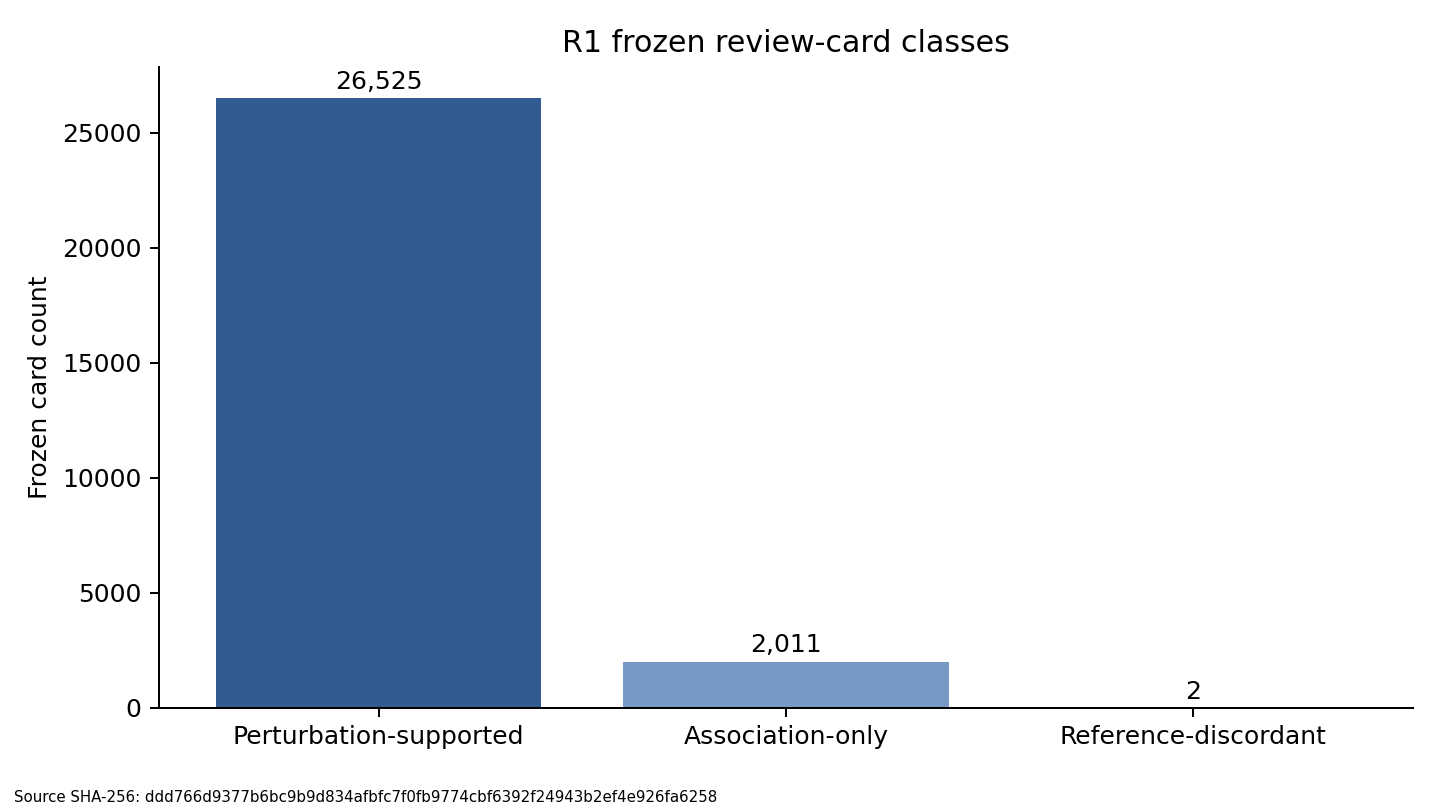
\includegraphics[width=0.82\linewidth]{../figures/r1_card_counts.png}\end{center}The frozen queue has three classes. Perturbation-supported contains 26,525 rows. Association-only contains 2,011 rows under the frozen $|r|\ge0.5$ definition. Reference-discordant contains two sign contradictions preserved rather than resolved. The card TSVs are included byte-for-byte. This figure is a deterministic rendering of \texttt{review\_queue\_summary.json}; its source hash is embedded in the PNG and recorded in a sidecar. It adds no analysis.\src{results/review\_queue\_summary.json; results/cards\_*.tsv; figures/r1\_card\_counts.SOURCE.sha256}}\newpage

\pg{8. The 26,525 review-edge definition}{The phrase ``26,525 review edges'' is shorthand for the exact 26,525 rows in \texttt{cards\_perturbation\_supported.tsv}. Each row is a target--gene review card from the strict 118-target K562 cohort. It passed all three frozen criteria: absolute score above 0.269, a 95\% construct confidence interval excluding zero, and an absolute per-gene NTC-null z score of at least 1.96. The median supported count was 142.5 per target and the tenth percentile was 29.7.\par\boxnote{Caveats carried with the count: exploratory calibration history; pooled cell-state estimate; no per-state claim; incomplete reference coverage; no graph claim; no causal-edge claim; no transport claim; unlisted edges are unlabeled, not negative; paired-guide halves are not independent replicates.}\src{results/supported\_final.json; results/gate\_evaluation\_r1.json; results/cards\_perturbation\_supported.tsv}}\newpage

\pg{9. Reference and LINCS stop grounds}{Only 31 of 118 primary targets were CollecTRI or OmniPath sources. The frozen audit universe $E^*$ contained 142 edges across 25 evaluable targets, below the locked graph-work floor. Reference resources are incomplete, so absence never became a negative label.\par The LINCS Level-5 archive was 21,328,033,748 bytes while the environment had 15 GB free. Anonymous access to the named S3 route returned AccessDenied; the gzip archive was not range-sliceable; iLINCS was a different aggregation and not a substitute under the lock. This was an environmental nontransport result, not evidence against biological transport.\src{results/reference\_audit.json; results/e\_star\_audit\_universe.json; results/gate\_evaluation\_r1.json; data\_manifest/lincs\_sha256\_manifest.txt}}\newpage

\pg{10. R2 setup}{RPE1 cohorts were built independently under the same construct and QC rules. The strict RPE1 cohort contained 135 targets; the descriptive tier contained 2,016; there were 11,485 NTC cells across 56 batches. The frozen request for 80 pools of 177 controls was infeasible because 14,160 controls would have been required. The documented adaptation used $\min(80,\lfloor11485/177\rfloor)=64$ pools, with the seed and threshold formula unchanged. RPE1 $\tau$ was 0.2360598147, and 87,880 RPE1-supported edges were recorded.\par The cross-line comparison was frozen over 115 shared strict targets and 7,226 shared genes. All shared genes passed the frozen stratum-A constitutive-expression rule; no stratum-B claim was made.\src{report/r2\_report.md; results/rpe1\_tau.json; results/r2\_rpe1\_freeze\_manifest.json; results/r2\_shared\_overlap\_freeze.json}}\newpage

\pg{11. R2 transport results}{\begin{center}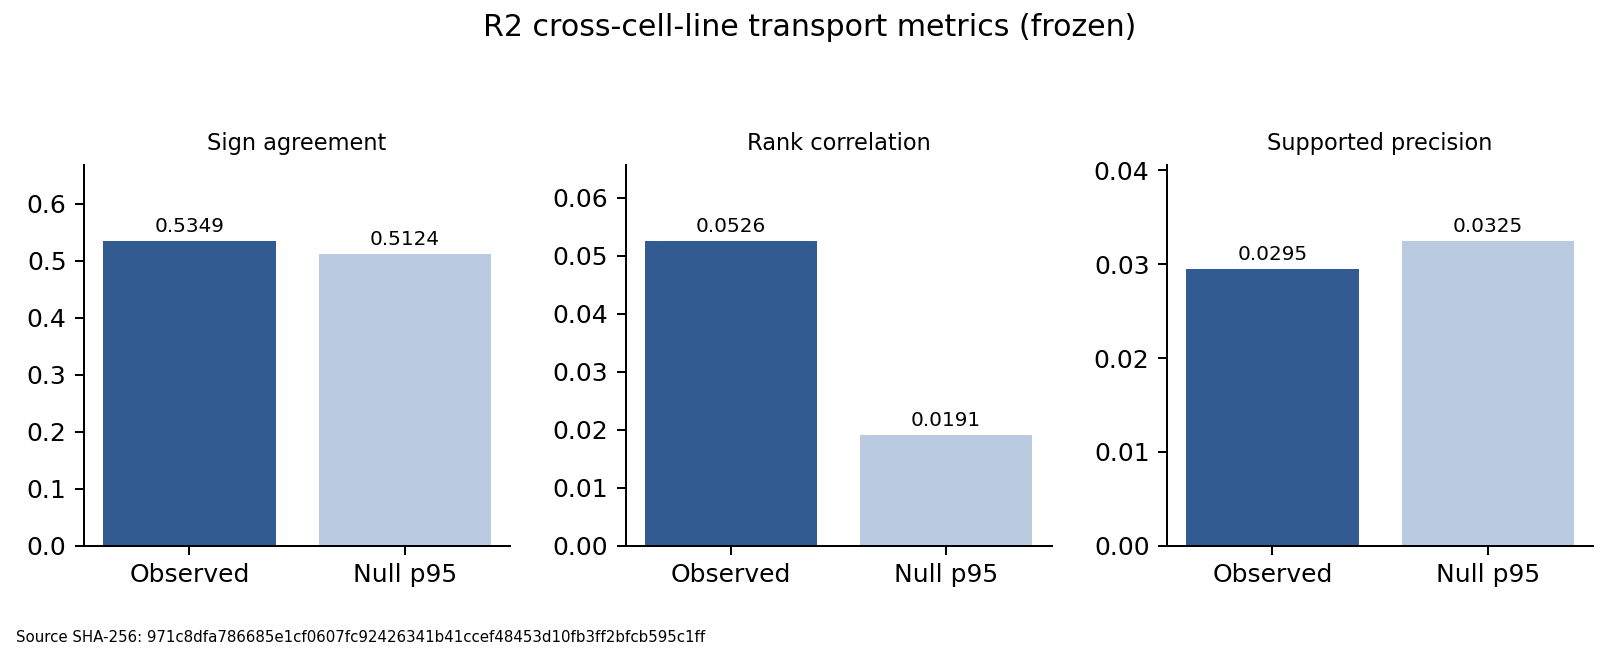
\includegraphics[width=0.92\linewidth]{../figures/r2_transport_metrics.png}\end{center}Sign agreement was 0.5349 with bootstrap interval 0.5275--0.5428, compared with a target-permuted null p95 of 0.5124 and an expression-matched null of 0.5256. Median Spearman rank correlation was 0.0526, interval 0.0514--0.0542, compared with null p95 0.0191. Supported-set precision was 0.0295, interval 0.0239--0.0357, compared with null p95 0.0325. Because the precision interval did not clear the required null boundary, the locked composite transport rule failed.\src{results/r2\_transport\_evaluation.json; figures/r2\_transport\_metrics.SOURCE.sha256}}\newpage

\pg{12. R2 interpretation}{Whole-transcriptome direction and rank contained weak nonzero cross-line structure. The expression-matched sign null was nearly equal to observed sign agreement, which cautions against treating directionality as target-specific biology. The discrete supported-edge decisions, the object shipped by the R1 queue, did not reproduce beyond chance under the locked precision criterion. Supported-set recall was 0.0875 and Jaccard was 0.0182. The fraction of K562-supported edges also supported in RPE1 was 10.96\%, compared with a 2.73\% target-permuted null rate; this enrichment was not sufficient to pass the locked rule.\par\boxnote{Verdict: TRANSPORT FAIL. R1 remains a K562-only exploratory and bounded review-queue atlas.}\src{results/r2\_transport\_evaluation.json; report/r2\_report.md}}\newpage

\pg{13. Card schemas}{\textbf{Perturbation-supported:} target, gene, class, score, construct\_se, null\_z, assoc\_r.\\\textbf{Association-only:} target, gene, class, assoc\_r, score, null\_z.\\\textbf{Reference-discordant:} target, gene, class, reference\_sign, observed\_score, null\_z, note.\par Values are retained as text exactly as stored in the TSVs. The packaged CLI exposes schema and exact-row query commands and exports a whole class in one stable lexical order. It does not add a score order or choose a subset.\par The separate schemas matter: missing columns must not be inferred across classes. A reference-discordant row is a preserved contradiction and is not automatically either a positive or negative validation record.\src{results/cards\_association\_only.tsv; results/cards\_perturbation\_supported.tsv; results/cards\_reference\_discordant.tsv}}\newpage

\pg{14. Read-only tool}{The package includes \texttt{cli/doc2033\_review.py}, implemented with the Python standard library. It provides \texttt{summary}, \texttt{schema}, exact \texttt{lookup}, fixed stable \texttt{row}, full-class \texttt{export}, and \texttt{verify}. It has no threshold argument, no score sort, no ranking, no filtering, no model call, no network call, and no file-write path.\par Golden tests compare canonical output byte-for-byte. A full association-only export is run twice to check determinism. Corruption testing changes a frozen result in a temporary copy and requires verification to fail. The manifest check is bidirectional: listed hashes must match, and unlisted extra bytes are rejected.\src{cli/doc2033\_review.py; cli/README.md; tests/run\_tests.py; tests/golden/}}\newpage

\pg{15. Provenance chain}{The scientific source tree is \texttt{projects/SP-007-DOC-2-033} at repository commit \texttt{7289559057802d5dbcea4e6bc46cea3e8c2cf19c}. Frozen protocol locks retain their original SHA-256 values. The package copies the full deliverables tree without changing scientific files, then adds report source/PDF, two deterministic figures and source-hash sidecars, the read-only CLI and tests, provenance notes, source-hash map, manifest, and closeout records.\par The source-hash map records every copied frozen file and compares its package hash with the source-tree hash. The clean-restore procedure runs in a new temporary directory from the archive bytes only: unpack, manifest verification, CLI verification, tests, PDF page-count check, and source-map check.\src{provenance/SOURCE\_HASH\_MAP.tsv; provenance/PROVENANCE.md; closeout/CLEAN\_RESTORE\_EVIDENCE.txt}}\newpage

\pg{16. External source matrices}{Large source matrices are not duplicated. The K562 harmonized matrix is \texttt{ReplogleWeissman2022\_K562\_essential.h5ad}, 1,546,729,675 bytes, MD5 \texttt{d8cba17576d1a8afc0f7d71b79cad0f7}, from Zenodo record 10044268. The RPE1 matrix is \texttt{ReplogleWeissman2022\_rpe1.h5ad}, MD5 \texttt{cc7f1ec50aeb3a3e1b4a6cfa713d80fa}, from the same record. The canonical raw K562 file is separately registered with provider MD5 \texttt{4f1122ce1c7f13299a68df6459a266d3}. Reference-table and LINCS hashes remain in the frozen manifests and environment ledger.\par These identifiers are external references only. A clean package restore does not recreate or substitute matrices and does not claim that the scientific pipeline can be rerun from the compact package alone.\src{protocol/provenance\_ledger.json; data\_manifest/h5ad\_md5\_manifest.txt; data\_manifest/lincs\_sha256\_manifest.txt}}\newpage

\pg{17. Environment and reproducibility notes}{The frozen analysis environment recorded Python 3.10.12 on Linux x86\_64 with anndata 0.11.4, h5py 3.16.0, scikit-learn 1.7.2, numpy 2.2.6, pandas 2.3.3, and scipy 1.15.3. Wheel hashes are retained in the frozen environment ledger. The R1 report records that an accumulation rerun reproduced an identical SHA-256. The R2 report states that the deterministic pipeline was identical in form to R1.\par The packaging environment is distinct and requires only Python standard library for the CLI/tests and pdfLaTeX for the report. The deterministic figures use only frozen JSON values; their source hashes are recorded. Package verification does not invoke scientific analysis code.\src{protocol/environment\_ledger.json; report/r1\_report.md; report/r2\_report.md; provenance/ENVIRONMENT.md}}\newpage

\pg{18. Limitations and honest negatives}{The atlas is confined to the K562 context and its recorded cohort. Cell-state sensitivity remained underpowered and is marked REVIEW. Multi-perturbation sensitivity was vacuous in the harmonized targeting cells. Reference coverability was below the graph-work floor. LINCS transport was not executed in the available environment. RPE1 supported-set precision did not pass. Same-lab/platform RPE1 is not independent replication. The descriptive tier has extensive single-construct uncertainty.\par Preserved failures include the naive stratum estimator and initial threshold calibration. Keeping them in the record prevents the final queue from appearing prospectively cleaner than it was. No missing scientific artifact has been recreated from memory.\src{report/r1\_report.md; report/r2\_report.md; provenance/MISSING\_ARTIFACTS.md}}\newpage

\pg{19. Audit and custody}{Custody is established by three layers. First, \texttt{MANIFEST.sha256} hashes every regular package file except itself, with the archive hash as outer custody. Second, \texttt{SOURCE\_HASH\_MAP.tsv} maps copied frozen bytes back to the repository tree. Third, clean-restore evidence records verification from transferred archive bytes in a new temporary directory.\par Release requires the report, manifest, all irreplaceable bytes, and readback hashes to travel together. The outer archive hash, byte size, restored checks, and PDF page count are in the closeout evidence. Repository commit and Drive upload are deliberately outside this package-creation step and await independent auditor approval.\src{MANIFEST.sha256; provenance/SOURCE\_HASH\_MAP.tsv; closeout/CLEAN\_RESTORE\_EVIDENCE.txt; closeout/CLOSEOUT\_LEDGER.md}}\newpage

\pg{20. Submission checklist and conclusion}{\begin{itemize}\item Combined R1/R2 report and source included.\item Core conclusion preserved: K562 exploratory/bounded; RPE1 transport failed.\item Frozen protocols, reports, cards, tables, code, and audit records included.\item New figures trace to frozen JSON hashes and add no analysis.\item Read-only query/export CLI has no scoring, ranking, filtering, model, or threshold interface.\item Golden, determinism, corruption, extra-file, manifest, and restore checks recorded.\item Large source matrices remain external hash references.\item Source-hash map, package manifest, and closeout ledger included.\end{itemize}\boxnote{Conclusion. DOC-2-033 provides a bounded K562 review queue with explicit uncertainty and a negative cross-cell-line transport result. Its value is in auditable prioritization and in a clearly drawn portability boundary, not in a general causal atlas claim.}\src{PACKAGE\_MANIFEST.json; closeout/CLOSEOUT\_LEDGER.md}}\end{document}
